\documentclass{article}

\usepackage[utf8]{inputenc}
\usepackage{mathtools, amssymb}
\usepackage{caption}
\usepackage{subcaption}
\usepackage{graphicx}
\usepackage{booktabs}
\usepackage{wrapfig}

\graphicspath{ {./images/} }

\DeclarePairedDelimiter{\abs}{\lvert}{\rvert}
\DeclarePairedDelimiter{\norm}{\lVert}{\rVert}

\newcommand*\mean[1]{\bar{#1}}

\title{Learn to Scale}
\author{alex.kreimer, ilan.shimshoni}
\date{May 2016}

\begin{document}

\maketitle

\begin{abstract}
  The size of a translation vector for a single moving camera is not
  directly observable, although is desirable.  Stereo, scene/camera
  prior assumptions were used in the past to recover the translation
  size.  We argue that the required information is present in the
  images and explore a number of ways to learn it.  We experiment with
  both ``legacy'' shallow learning methods and hand-crafted features
  as well as end-to-end learning methods based on the convolutional
  neural networks.
\end{abstract}

\section{Introduction}

Recovering camera 6-DOF ego-motion from images is a well studied
problem. It arises in various practical contexts
(e.g. virtual/augmented reality application, autonomous or aided
navigation, etc.).  The problem was studied in both stereo and the
monocular setups.  To recover the full 6-DOF motion, the previous
works resorted to the stereo setup, used auxiliary sensors (e.g. IMU)
or made assumptions about the camera pose and the scene.  All of these
have their drawbacks: stereo pairs are fragile and require careful
calibration procedures, additional sensors are not always available
and also require calibration, scene assumptions don't always hold.
Motion estimation from images of a single moving camera is probably
the hardest setup, as well as the most desirable one, because of its
simplicity.  It is well known that the translation scale parameter is
not directly observable for a motion of a single camera.

We argue, that for natural scenes the scale information is present in
the images and may be extracted.  Our method learns a regressor, that
is capable to prediction the motion scale.

\section{Related work}

\subsection{Others}
\subsection{Our method}

We assume that a single camera moves through space and takes images.
We treat the initial camera pose (at time $t=0$) as the world
coordinate frame.  We denote the pose of the camera at time $t$ by
$\mathbf{\hat{T}}_t$ described by the rotation matrix
$\mathbf{\hat{R}}_t$ and the translation vector $\mathbf{\hat{t}}_t$
as seen in the world coordinate frame.  We denote camera image taken
at time $t$ by $I_t$.  To facilitate the discussion, we also introduce
notation for camera pose
$\mathbf{T}_t = [\mathbf{R}_t\ |\ \mathbf{t}_t] $ as seen from the
coordinate frame associated with camera pose at time $t-1$.  Most of
the time, we will omit the time index, since its clear from the
context.  By translation scale (or simply, scale) we refer to the norm
of the translation vector $\mathbf{t}$ (e.g.,
$s = \lVert \mathbf{t} \rVert$)

We pose the scale estimation problem as a regression problem and
search for a good regressor model.

\section{Random forest}

\subsection{Decision trees}

In this section we briefly describe tree-based methods for regression.
These involve splitting the feature space into a number of small
regions.  The prediction for a sample is made by computing a mean or a
mode of training samples that belong to the same region.  Since the
set of rules used to split the feature space into smaller regions may
be described by a tree, these methods are referred to as
\textit{decision tree} methods.

Building a decision tree may be described by a two step procedure:
\begin{enumerate}
\item Split the feature space, e.g., the set of all possible values
  for $X_1, X_2,\ldots,X_n$ into $J$ distinct regions $R_1, R_2,\ldots, R_J$.
\item For every sample that belongs to the regions $R_i$ we make the
  same prediction, which is a mean of the responses of training
  samples that belong to this region.
\end{enumerate}

The regions $R_i$ are usually chosen to be multidimensional boxes (axis aligned).  We would like to find such a partition of the feature space that minimizes
\begin{equation}\label{eq:tree_objective}
\sum\limits_{j=1}^J\sum_{x\in R_j}{(x-\mean{x}_j)^2}
\end{equation}

Where $\mean{x}_j$ denotes the mean of the response values of the
samples in region $R_j$.  Unfortunately, solving the optimization
problem~\ref{eq:tree_objective} is computationally hard.  Usually it
is replaced with a greedy algorithm, called \textit{recursive binary
  splitting}.  This approach starts at the top of the tree and
greedily chooses the best split at that point that minimizes the
variance of its sub-trees.  To be more precise, for each $j$ and $s$ we
define the hyper-planes:

\begin{equation}
  R_1(j,s) = \{ X\lvert X_j<s \}\quad\text{and}\quad R_2(j,s) = \{ X\lvert X_j \geq s \},
\end{equation}

We seek such $j$ and $s$ that minimize the equation:

\begin{equation}
  \sum\limits_{i:x_i\in R_1(j,s)}{(y_i-\hat{y}_{R_1})}^2 + \sum\limits_{i:x_i\in R_2(j,s)}{(y_i-\hat{y}_{R_2})}^2,
\end{equation}

Where $y_{R_1}, y_{R_2}$ are the average responses of the samples in
$R_1(j,s), R_2(j,s)$ respectively.  Once we found the $j$ and $s$ we
recursively split each sub-tree in a similar manner.  The process is
repeated until stopping criterion (e.g., number of nodes in the leaf)
is reached.

\subsection{Bagging}
The decision trees tend to suffer from \textit{high variance}. This
means that if we split the training set into a number of random
subsets and fit random tree into each sub-sample, we would likely to
get much different answers from these trees when asked the same
question.  It is known that the variance of a mean of a set of
independent random variables is $\frac{1}{n}$.  Thus, in order to
improve the variance of the estimator, it is possible to fit $n$
estimators, each to its training-set and the average their
predictions.  Since, usually, we don't have $n$ training sets, we
would use \textit{bootstrapping} (e.g., sample independently with
replacement from the data set).

\subsection{Random Forest}
Random forest suggest additional improvement over bagging, by
decorrelating the random trees.  The issue they attempt to address is
this: lets say there is a very dominant feature w.r.t. to task at hand
for a given data-set.  Bagging ensures that we use different training
sets, but yet, most trees will tend to first split on this dominant
feature.  In this case the trees will resemble each other.  In random
forest, the trees are constructed by using only a subset of features
(e.g., $m = \sqrt{p}$).  This means that at calculating the splits,
the algorithm is allowed to consider only a subset of features.

\section{Convolutional Neural Networks}

Convolutional neural networks (CNN) leverage the availability of the
computational power and the abundance of data.  CNN have become a
method of choice in a number of computer vision areas (e.g., image
classification, object recognition).  They were also shown capable of
per-pixel tasks, such as semantic segmentation and depth estimation
from a single image. Works like (e.g., flownet) show that CNN can do
well for task that require feature matching as well as feature
extraction.

With these encouraging works in mind, we turn to CNN for our task.
There are lots of network architectures out there to choose from. We
have decided to use the ZF~\cite{DBLP:journals/corr/ZeilerF13} object
recognition network as a basic building block for our work.

The network architecture consists of 5 convolutional layers, kernel
sizes 7, 5, 3, 3, 3.  Four initial convolutional layers are each
followed by the relu, max-pooling and local response normalization
operations.  Conv5 is followed by two fully connected layers separated
by non-linearity.  The fully connected layers are of size
4096. Finally, there is a last fully connected layer that reduced the
network to a single output, which we are interested to learn.  We use
euclidean loss to train the network.

\section{Recurrent Neural Networks}

Many problems require passing information through time.  Since the
traditional neural networks are stateless, they are poorly suited for
this purpose. Recurrent Neural Networks have loops in them, so that
the information can persist.

\begin{figure}[h!]
  \centering 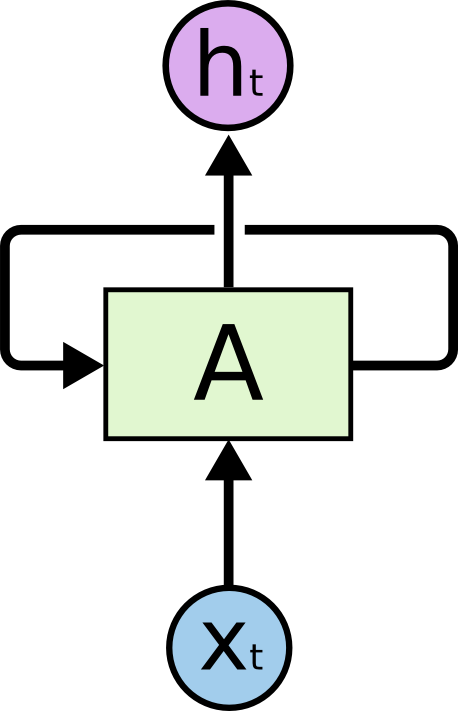
\includegraphics[width=0.15\textwidth]{RNN-rolled}
  \caption{RNN}
  \label{fig:rnn1}  
\end{figure}

In the Figure~\ref{fig:rnn1} network $A$ accepts input $x_t$ and
outputs $h_t$.  The loop allows the network to pass information from
one step of to another.

The RNN may be thought of as a chain of multiple copies of the same
neural network where each node passes a message to its successor.
This is called \textit{network unrolling}, depicted in
Figure~\ref{fig:rnn2}.  Unrolled network stresses the relation of the
RNN to the sequential data streams.  This is an architecture of choice
when modeling such data.

\begin{figure}[ht!]
  \centering 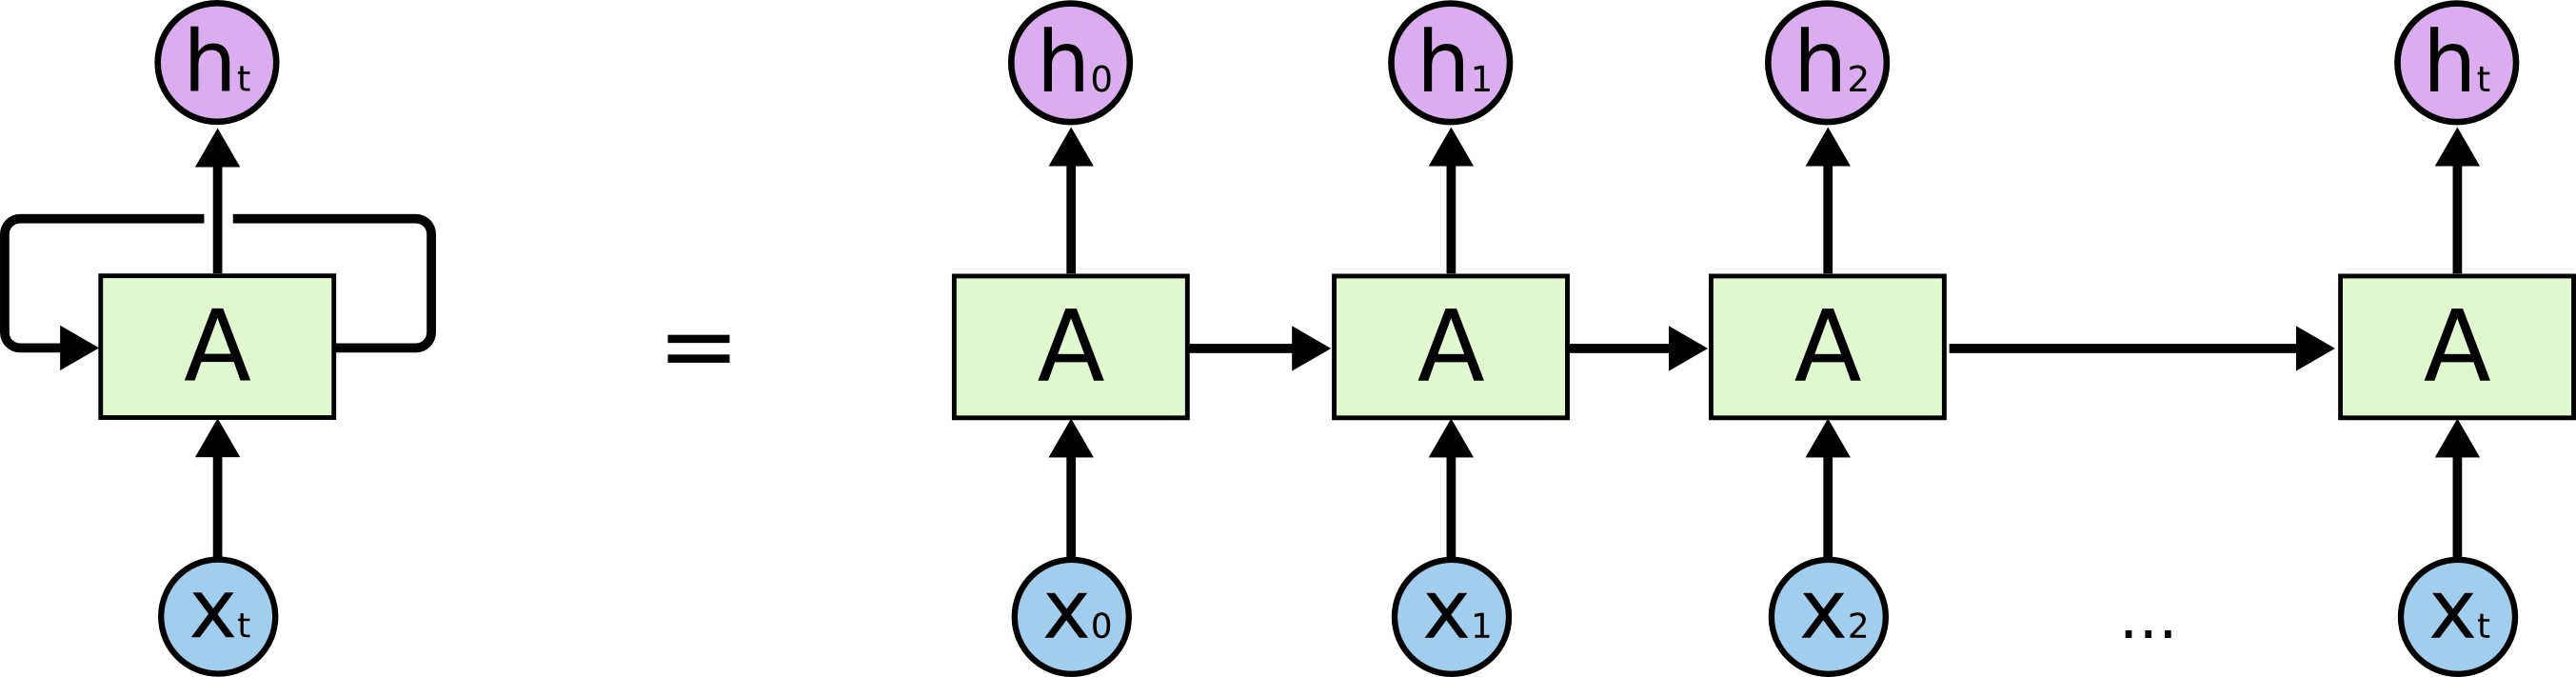
\includegraphics[width=.7\textwidth]{RNN-unrolled}
  \caption{An unrolled RNN}\label{fig:rnn2}
\end{figure}

It turns out that the vanilla RNN are hard to train due to the
exploding/imploding gradients.  Fortunately, Long Short Term Memory
Networks (LSTM), which is a special kind of RNN addresses these issues.

LSTM were introduced by~\cite{hochreiter1997long}, they are
specifically designed to model long term dependencies. Similarly to
RNN, LSTM posses a chain-like structure. Each repeating node has an
internal structure depicted in Figure~\ref{fig:lstm1}.

\begin{figure}[ht!]
  \centering 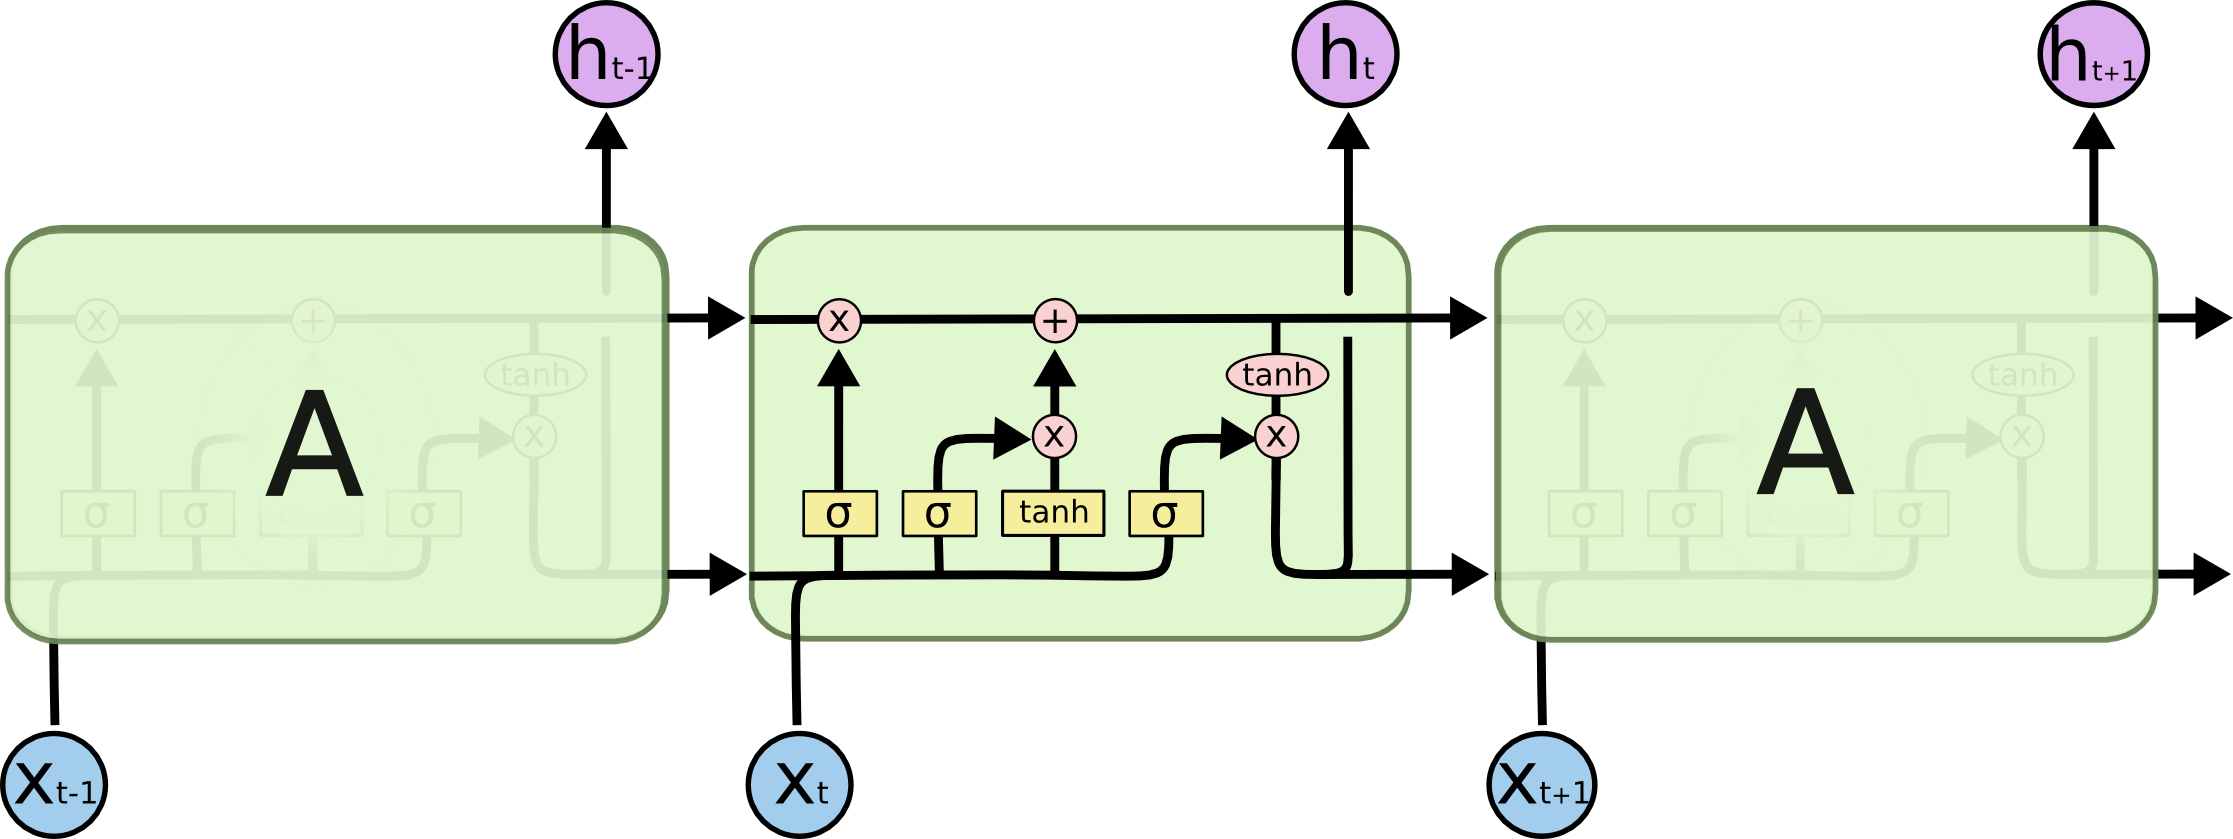
\includegraphics[width=.7\textwidth]{LSTM3-chain}
  \caption{Long Short Term Memory}\label{fig:lstm1}
\end{figure}

\begin{figure}[ht!]
  \centering 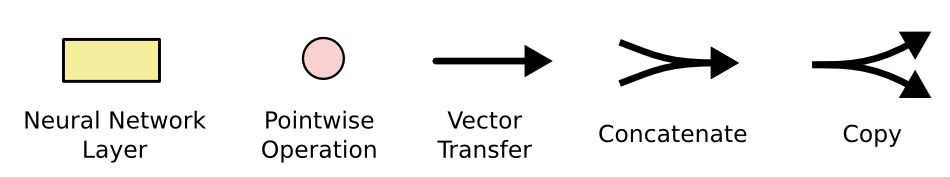
\includegraphics[width=.5\textwidth]{LSTM2-notation}
  \caption{A notation used in Figure~\ref{fig:lstm1}}\label{fig:lstm2}
\end{figure}

To use the LSTM for the image data we combine the convolutional
network with the LSTM.  $X_t$ vectors are produced by the ZF convnet.
This is a fairly common representation used previously.  The convnet
and the LSTM are trained jointly.

\section{Experiments}

\subsection{Data-set}

We train and test on the KITTI data-set~\cite{geiger2013vision}.  The
data-set consists of 11 sequences with ground truth data.  We
arbitrarily use sequence 00 for testing and sequences 01-10 for
training.  There are 4540 and 18650 images in the test and the train
sets respectively. We only use the data from the left color camera.
Figure~\ref{fig:scales} depicts the distribution of the scale values
over the train and the test sets.

\begin{figure}[!ht]
  \begin{subfigure}{0.5\textwidth}
    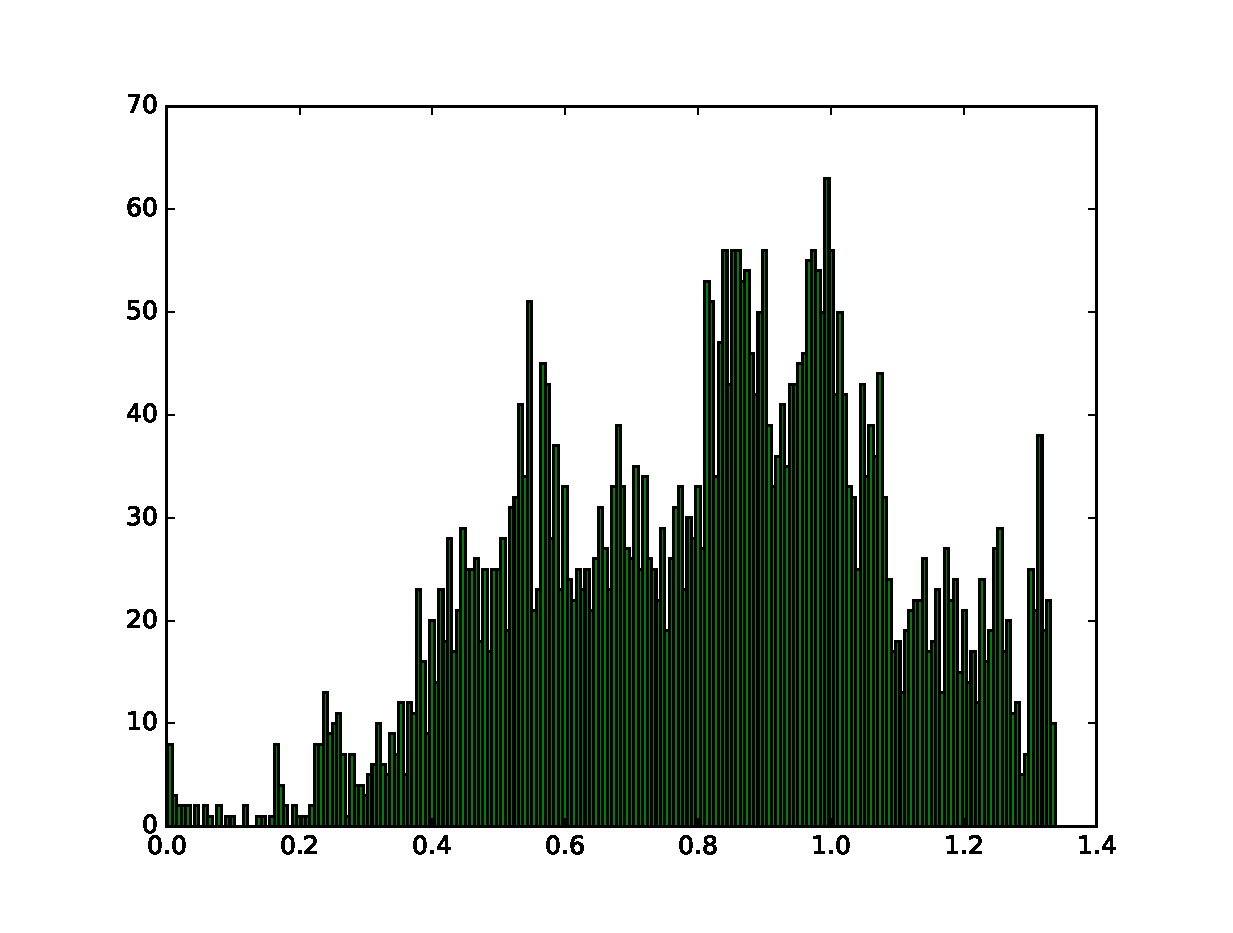
\includegraphics[width=0.9\linewidth]{00-scales}
    \caption{The test set}		
    \label{fig:stats-00}
  \end{subfigure}
  \begin{subfigure}{0.5\textwidth}
    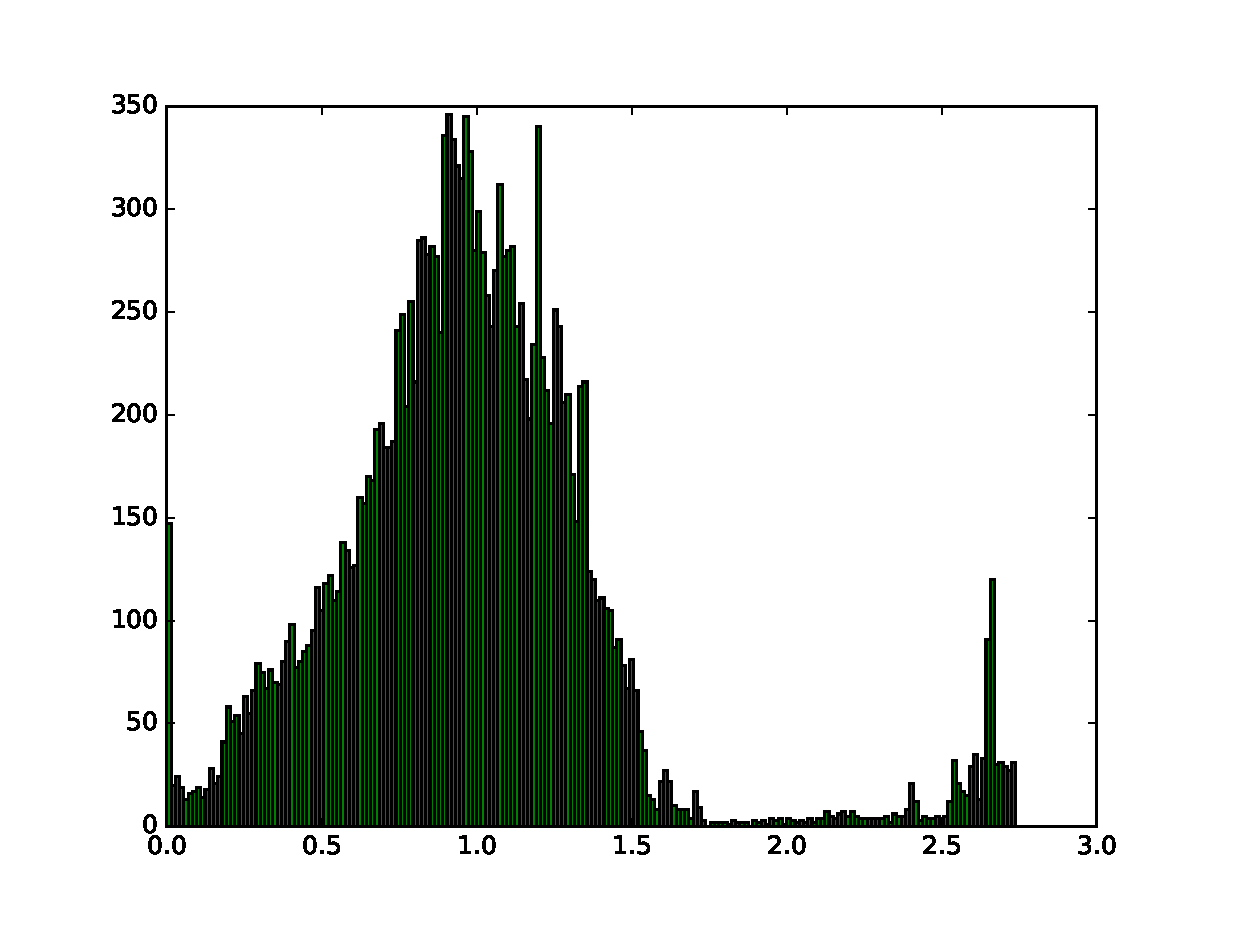
\includegraphics[width=0.9\linewidth]{no_00-scales}
    \caption{The train set}
    \label{fig:stats-no_00}
  \end{subfigure}
  \caption{Scale distributions}
  \label{fig:scales}
\end{figure}

\subsection{Random Forest}

\subsection{Feature Extraction}\label{sec:features}

In order to train the random forest we need to represent subsequent
image pairs as feature vectors, which are created as follows: we
extract and match sparse salient points in both input images.  The
output of this stage is a set of a corresponding pixel locations.
Then, we compute the point displacement magnitudes.  Finally, we bin
all the interest pundits according to a grid and create histogram of
displacement magnitudes for each bin.  Concatenating all histograms
together produces a feature vector. We use Harris corners and square
$11\times 11$ patches as corner descriptors. Sum of square differences
is used as a distance measure with the winning pair declared a match.
To prune the outliers we fit the fundamental matrix into the matched
corner sets and remove the corners that do not agree with the model.
Figure~\ref{fig:ex_corner_and_matching} shows a typical example of
extracted and matched corners.


Some statistics of the features is presented in the
Figure~\ref{fig:feature_vectors}. We expect the peaks, that correspond
to a closer image regions have a distributions shifted to the right
(i.e., larger displacements) and the peaks that correspond to a
regions farther away should be closer to zero.  This behavior can be
observed especially well for the feature vectors that correspond to
larger camera displacements (e.g. Figure~\ref{fig:1c}).

\begin{figure}[!ht]
  \centering
  \begin{subfigure}{.45\linewidth}
    \centering
    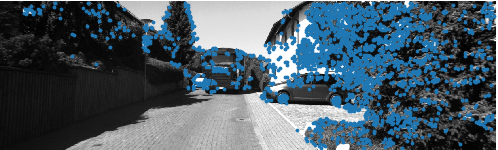
\includegraphics[width=\linewidth]{10_001157_001158_raw_corners_left}
    \caption{}
    \label{fig:ex_corner_and_matching:corner}
  \end{subfigure}
  \begin{subfigure}{.45\linewidth}
    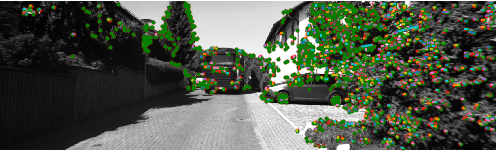
\includegraphics[width=\linewidth]{10_001157_001158_final_matches1}
    \caption{}
    \label{fig:ex_corner_and_matching:match}    
  \end{subfigure}
  \caption{Typical corner extraction and
    matching. Figure~\subref{fig:ex_corner_and_matching:corner} shows the raw
    extracted corners, while Figure~\subref{fig:ex_corner_and_matching:match} shows
    pruned and matched corners.}
  \label{fig:ex_corner_and_matching}
\end{figure}

\begin{figure}[!ht]
  \centering
  \begin{subfigure}{.45\linewidth}
    \centering
    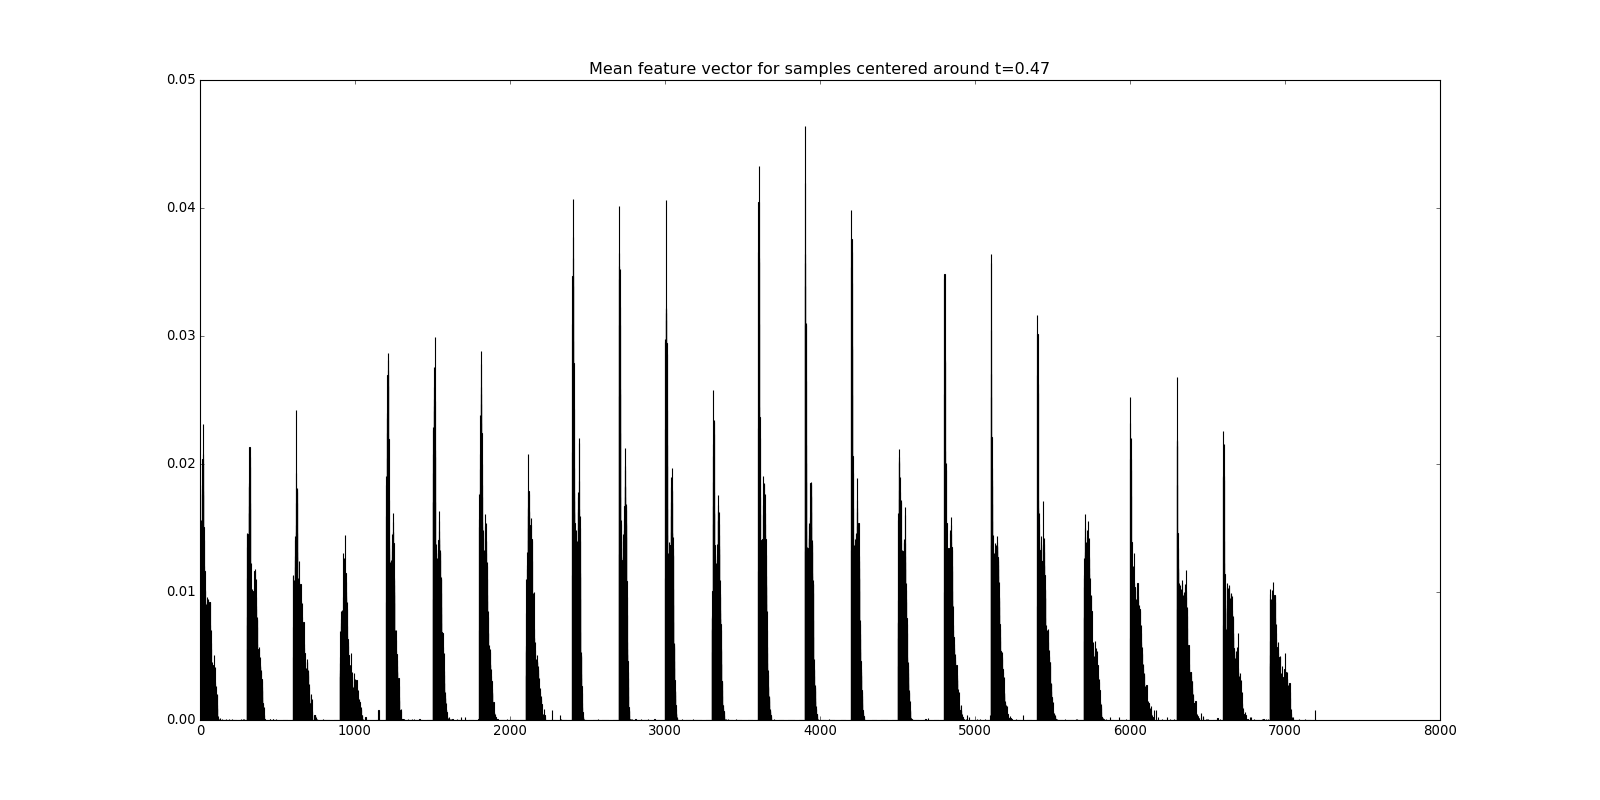
\includegraphics[width=1.2\linewidth]{00_mean_feature_vector_0_47}
    \caption{}\label{fig:1a}
  \end{subfigure}%
  \begin{subfigure}{.45\linewidth}
    \centering
    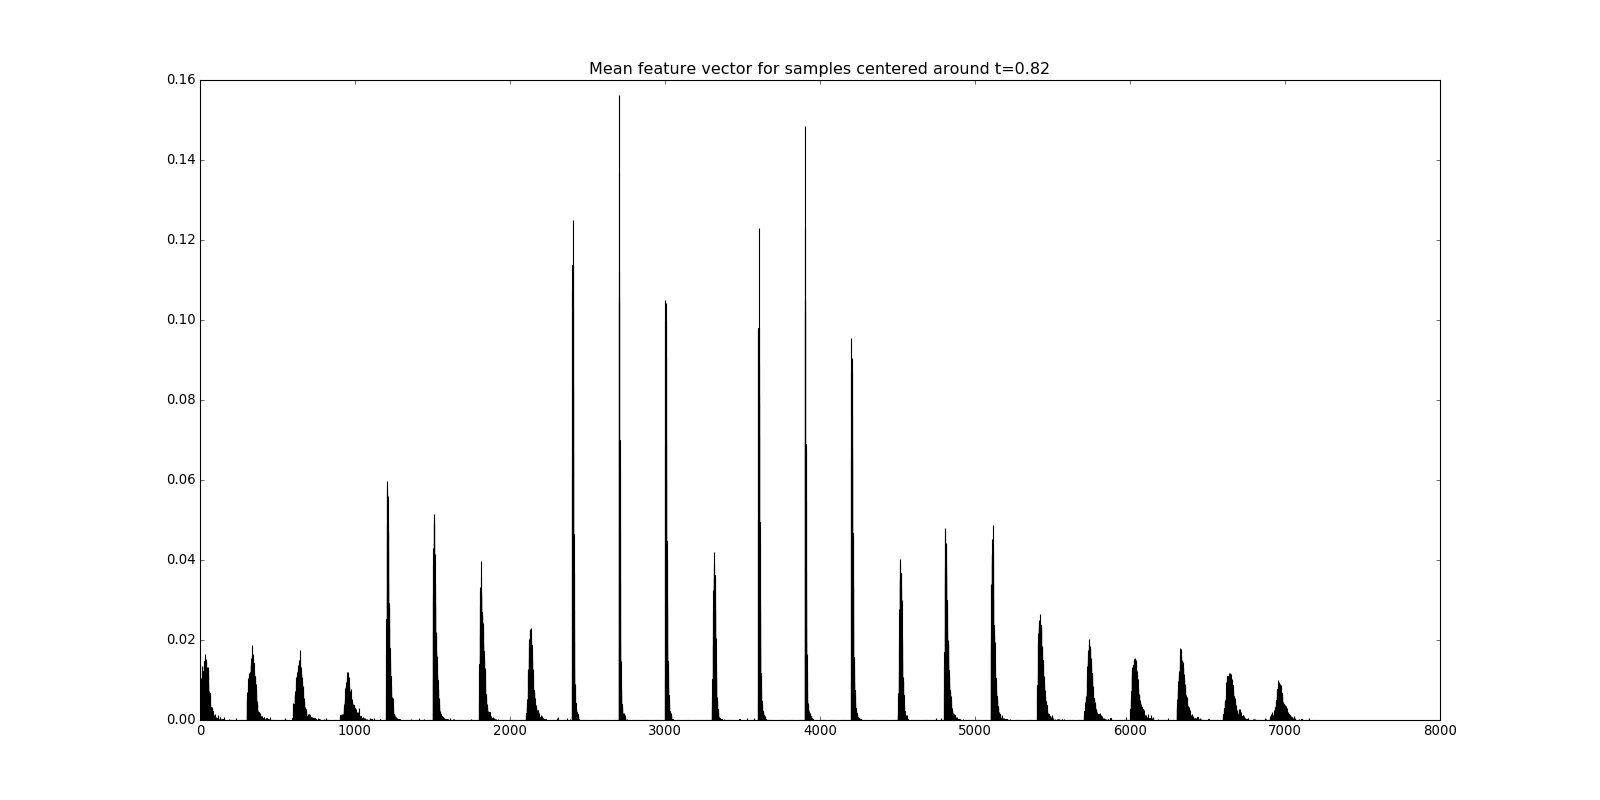
\includegraphics[width=1.2\linewidth]{00_mean_feature_vector_0_81}
    \caption{}\label{fig:1b}
  \end{subfigure}%
  \\
  \begin{subfigure}{\linewidth}
    \centering
    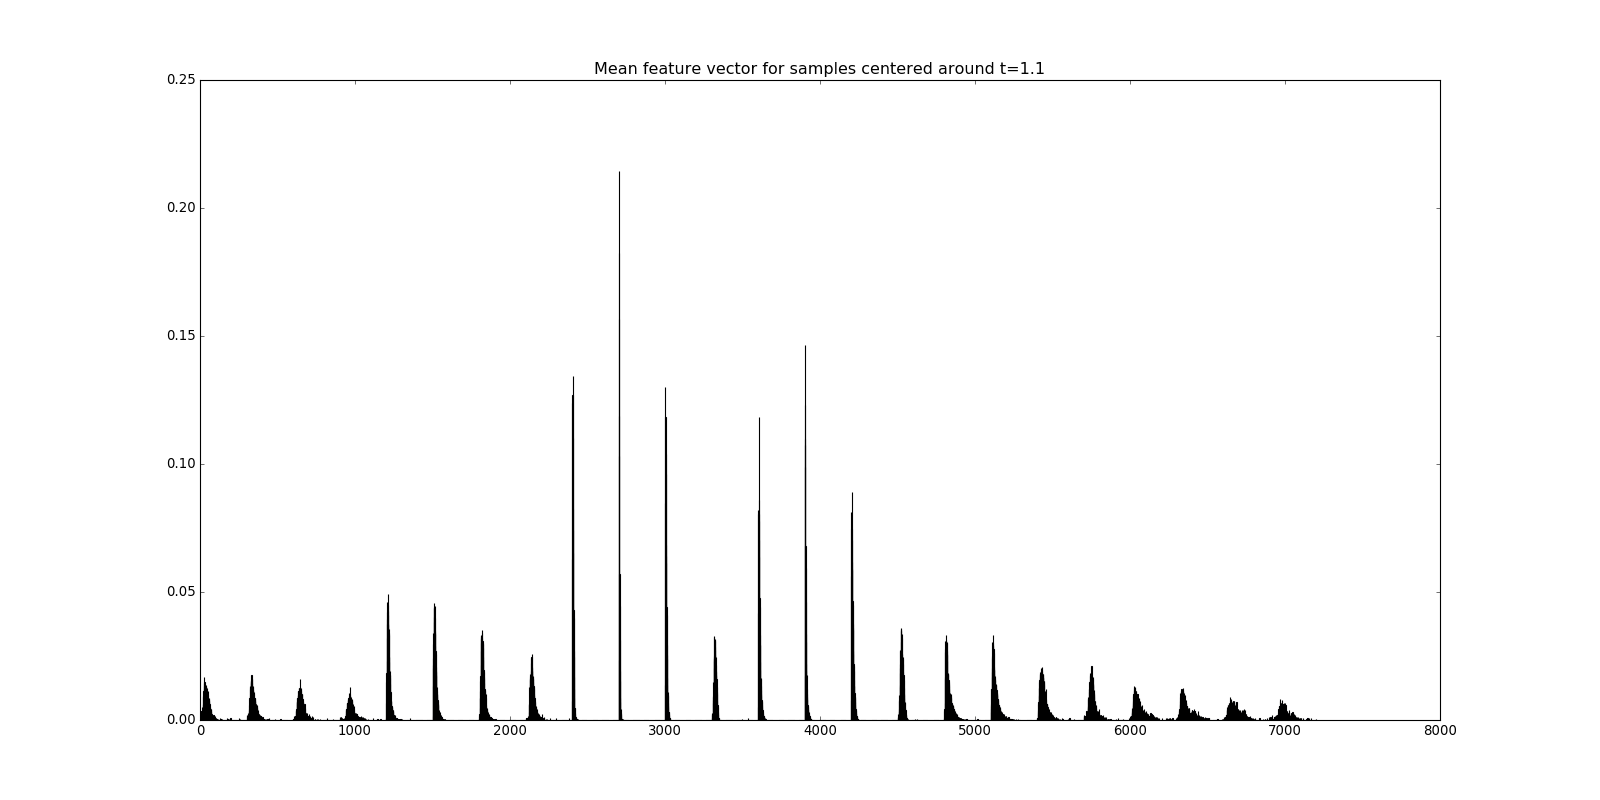
\includegraphics[width=.8\textwidth]{00_mean_feature_vector_1_1}
    \caption{}\label{fig:1c}
  \end{subfigure}%
  \caption{Average feature vectors for samples centered around the
    specific camera translation magnitude.  Each peak corresponds to a
    grid cell (e.g. here the grid is 4 rows by 6 columns by 300 bins,
    so the feature vector is of the dimension 6*4*300=7200).  The grid
    is sampled in a column-major mode. So the first four peaks
    correspond to the leftmost column of the image grid.}
  \label{fig:feature_vectors}
\end{figure}

We bin each image into $6\times 4$ grid.  For each bin in the image we
compute the histogram of corner disparities.  By disparity we denote
the displacement of the corner in the image.  We use $300$-bin
histogram for disparities (e.g, feature vector length is $7200$).

We use the extracted features to fit a random forest, by means of
recursive note splitting with sub-node variance minimization. The mean
absolute error is 0.237 meters with a standard deviation of=0.229
meters.  The visualization of a prediction is in the
Figure~\ref{fig:rf_fit}.

\begin{figure}[!ht]
  \centering
  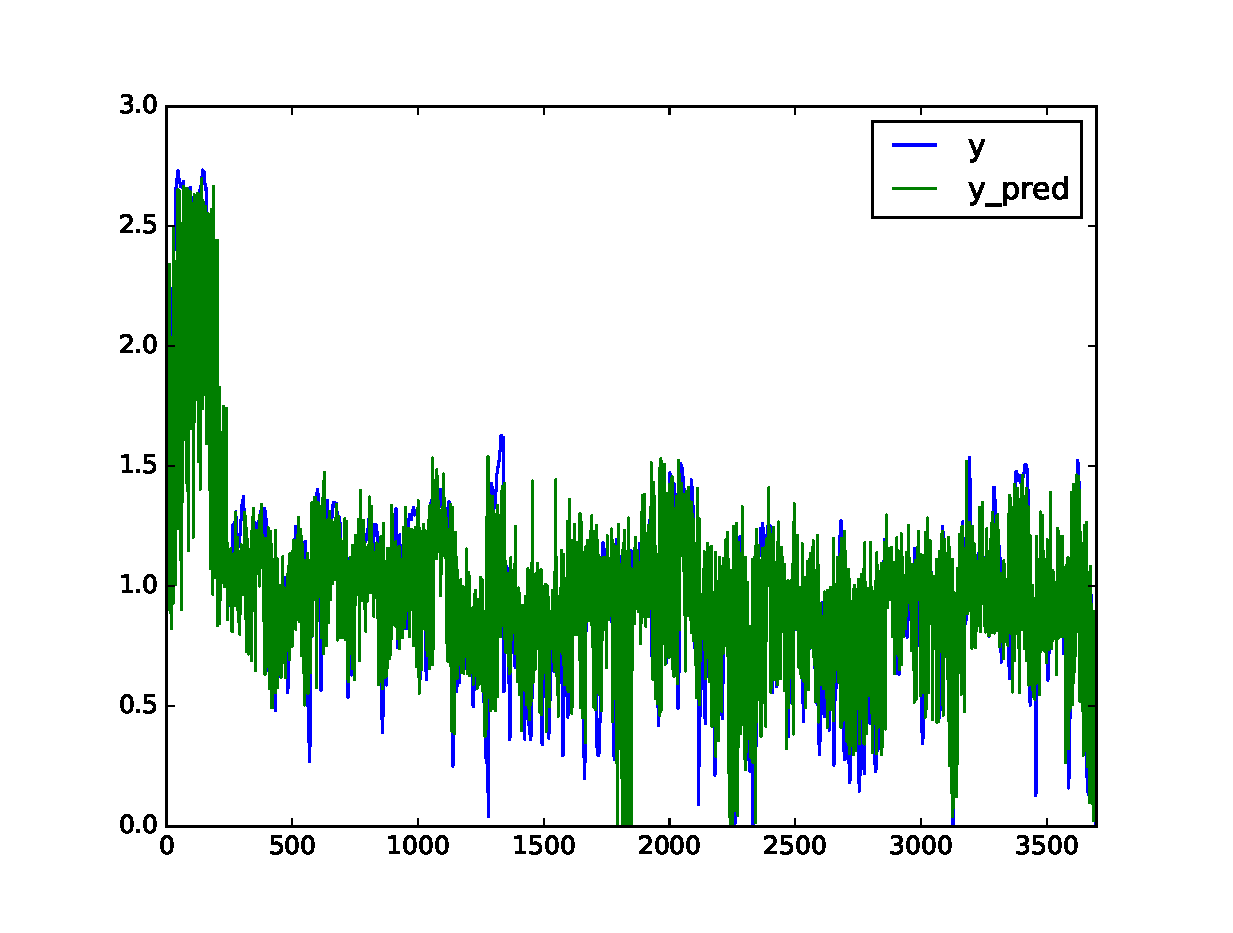
\includegraphics[width=1.2\linewidth]{yerr}
  \caption{Visualization of the random forest prediction}
  \label{fig:rf_fit}
\end{figure}

\section{Convolutional neural networks}

We use Caffe~\cite{jia2014caffe} framework to train and test our
models.

\section{LSTM}

\bibliographystyle{abbrv}
\bibliography{report_bib}

\end{document}

%%% Local Variables:
%%% mode: pdf
%%% TeX-master: t
%%% End:
